%-----------------------------------
% Define document and include general packages
%-----------------------------------
% Tabellen- und Abbildungsverzeichnis stehen normalerweise nicht im
% Inhaltsverzeichnis. Gleiches gilt für das Abkürzungsverzeichnis (siehe unten).
% Manche Dozenten bemängeln das. Die Optionen 'listof=totoc,bibliography=totoc'
% geben das Tabellen- und Abbildungsverzeichnis im Inhaltsverzeichnis (toc=Table
% of Content) aus.
% Da es aber verschiedene Regelungen je nach Dozent geben kann, werden hier
% beide Varianten dargestellt.
\documentclass[12pt,oneside,titlepage,listof=totoc,bibliography=totoc]{scrartcl}
%\documentclass[12pt,oneside,titlepage]{scrartcl}

%-----------------------------------
% Dokumentensprache
%-----------------------------------
%\def\FOMEN{}% Auskommentieren um die Dokumentensprache auf englisch zu ändern
\newif\ifde
\newif\ifen

%-----------------------------------
% Meta information
%-----------------------------------
%-----------------------------------
% Meta Informationen zur Arbeit
%-----------------------------------

% Autor
\newcommand{\myAutor}{Sebastian Bunge}

% Adresse
\newcommand{\myAdresse}{Lindenstra\ss e 15c \\ \> \> \> 53227 Bonn}

% Titel der Arbeit
\newcommand{\myTitel}{Development of a Query Language for Full-Text Search in Relational Databases}

% Betreuer
\newcommand{\myBetreuer}{Prof. Dr.-Ing. Peter Steininger}

% Lehrveranstaltung
\newcommand{\myLehrveranstaltung}{Modul}

% Matrikelnummer
\newcommand{\myMatrikelNr}{539441}

% Ort
\newcommand{\myOrt}{Bonn}

% Datum der Abgabe
\newcommand{\myAbgabeDatum}{\today}

% Semesterzahl
\newcommand{\mySemesterZahl}{7}

% Name der Hochschule
\newcommand{\myHochschulName}{FOM Hochschule für Oekonomie \& Management}

% Standort der Hochschule
\newcommand{\myHochschulStandort}{Bonn}

% Studiengang
\newcommand{\myStudiengang}{Wirtschaftsinformatik - Business Information Systems}

% Art der Arbeit
\newcommand{\myThesisArt}{Bachelor Thesis}

% Zu erlangender akademische Grad
\newcommand{\myAkademischerGrad}{Bachelor of Science (B.Sc.)}

% Firma
\newcommand{\myFirma}{Deutsche Telekom IT GmbH}


\ifdefined\FOMEN
    %Englisch
    \entrue
    \usepackage[english]{babel}
\else
    %Deutsch
    \detrue
    \usepackage[ngerman]{babel}
\fi


\newcommand{\langde}[1]{%
   \ifde\selectlanguage{ngerman}#1\fi}
\newcommand{\langen}[1]{%
   \ifen\selectlanguage{english}#1\fi}
\usepackage[utf8]{luainputenc}
\langde{\usepackage[babel,german=quotes]{csquotes}}
\langen{\usepackage[babel,english=british]{csquotes}}
\usepackage[T1]{fontenc}
\usepackage{fancyhdr}
\usepackage{fancybox}
\usepackage[a4paper, left=4cm, right=2cm, top=4cm, bottom=2cm]{geometry}
\usepackage{graphicx}
\usepackage{colortbl}
\usepackage[capposition=top]{floatrow}
\usepackage{array}
\usepackage{float}      %Positionierung von Abb. und Tabellen mit [H] erzwingen
\usepackage{footnote}
% Darstellung der Beschriftung von Tabellen und Abbildungen (Leitfaden S. 44)
% singlelinecheck=false: macht die Caption linksbündig (statt zentriert)
% labelfont auf fett: (Tabelle x.y:, Abbildung: x.y)
% font auf fett: eigentliche Bezeichnung der Abbildung oder Tabelle
% Fettschrift laut Leitfaden 2018 S. 45
\usepackage[singlelinecheck=false, labelfont=bf, font=bf]{caption}
\usepackage{caption}
\usepackage{enumitem}
\usepackage{amssymb}
\usepackage{mathptmx}
%\usepackage{minted} %Kann für schöneres Syntax Highlighting genutzt werden. ACHTUNG: Python muss installiert sein.
\usepackage[scaled=0.9]{helvet} % Behebt, zusammen mit Package courier, pixelige Überschriften. Ist, zusammen mit mathptx, dem times-Package vorzuziehen. Details: https://latex-kurs.de/fragen/schriftarten/Times_New_Roman.html
\usepackage{courier}
\usepackage{amsmath}
\PassOptionsToPackage{table}{xcolor}\usepackage[most]{tcolorbox}
\tcbset{standard jigsaw, opacityback=0, colframe=black, sharp corners}
\usepackage{marvosym}			% Verwendung von Symbolen, z.B. perfektes Eurozeichen
\usepackage{forest}
\usepackage[nounderscore]{syntax}	% Write proper Backus-Naur Form, no underscore is needed to avoid problems with the cite function
\setlength{\grammarindent}{0pt}	% No indent in grammar to not having to use paragraphs and waste space

\renewcommand\familydefault{\sfdefault}
\usepackage{ragged2e}

% Mehrere Fussnoten nacheinander mit Komma separiert
\usepackage[hang,multiple]{footmisc}
\setlength{\footnotemargin}{1em}

% todo Aufgaben als Kommentare verfassen für verschiedene Editoren
\usepackage{todonotes}

% Verhindert, dass nur eine Zeile auf der nächsten Seite steht
\setlength{\marginparwidth}{2cm}
\usepackage[all]{nowidow}

%-----------------------------------
% Farbdefinitionen
%-----------------------------------
\definecolor{darkblack}{rgb}{0,0,0}
\definecolor{dunkelgrau}{rgb}{0.8,0.8,0.8}
\definecolor{hellgrau}{rgb}{0.0,0.7,0.99}
\definecolor{mauve}{rgb}{0.58,0,0.82}
\definecolor{dkgreen}{rgb}{0,0.6,0}

%-----------------------------------
% Pakete für Tabellen
%-----------------------------------
\usepackage{epstopdf}
\usepackage{nicefrac} % Brüche
\usepackage{multirow}
\usepackage{rotating} % vertikal schreiben
\usepackage{mdwlist}
\usepackage{tabularx}% für Breitenangabe

%-----------------------------------
% sauber formatierter Quelltext
%-----------------------------------
\usepackage{listings}
\usepackage{listings-rust}

% linenumber fix for listings
\usepackage{etoolbox}% http://ctan.org/pkg/etoolbox
\makeatletter
\patchcmd{\lst@GLI@}% <command>
  {\def\lst@firstline{#1\relax}}% <search>
  {\def\lst@firstline{#1\relax}\def\lst@firstnumber{#1\relax}}% <replace>
\makeatother

\lstdefinelanguage{Fulltext-Search}{
	keywords={@contains, @startswith, @inflection, @thesaurus, @near, @weighted},
	ndkeywords={:, +, &, |, !, -},
	ndkeywordstyle=\color{darkgray},
	morestring=[b]"
}
\lstdefinelanguage{toml}{
	keywords={package, dependencies, name, version, edition},
	ndkeywords={[,],=},
	ndkeywordstyle=\color{darkgray},
	morestring=[b]",
	morecomment=[l]{\#}
}

\lstset{
	numbers=left,
	numberstyle=\tiny,
	numbersep=5pt,
	breaklines=true,
	showstringspaces=false,
	frame=l ,
	xleftmargin=5pt,
	xrightmargin=5pt,
	basicstyle=\ttfamily\small,
	stepnumber=1,
	keywordstyle=\color{blue},          % keyword style
  	commentstyle=\color{dkgreen},       % comment style
  	stringstyle=\color{mauve}         % string literal style
}

%-----------------------------------
%Literaturverzeichnis Einstellungen
%-----------------------------------

% Biblatex

\usepackage{url}
\urlstyle{same}

%%%% DIN 1505 Leitfaden
\usepackage[backend=biber, style=din, maxcitenames=2]{biblatex}%iso date format für YYYY-MM-DD

%% et al. anstatt u. a. bei mehr als drei Autoren.
\DefineBibliographyStrings{ngerman}{ 
	andothers = {{et\,al\adddot}},             
}
\DefineBibliographyStrings{english}{ 
	andothers = {{et\,al\adddot}},             
}

% Bib-Datei einbinden
% Replacement string for Zotero: \n\s+file = \{.*\},
\addbibresource{literature/literature.bib}

% Zeilenabstand im Literaturverzeichnis ist Einzeilig
% siehe Leitfaden S. 14
\AtBeginBibliography{\singlespacing}

%-----------------------------------
% Silbentrennung
%-----------------------------------
\usepackage{hyphsubst}
\HyphSubstIfExists{ngerman-x-latest}{%
\HyphSubstLet{ngerman}{ngerman-x-latest}}{}

%-----------------------------------
% Pfad fuer Abbildungen
%-----------------------------------
\graphicspath{{./}{./figures/}}

%-----------------------------------
% Weitere Ebene einfügen
%-----------------------------------
\usepackage{titletoc}

\makeatletter

% Setze die Tiefe des Inhaltsverzeichnis auf 4 Ebenen
% Damit erscheinen \paragraph-Sektionen auch im Inhaltsverzeichnis
\setcounter{secnumdepth}{4}
\setcounter{tocdepth}{4}

% Fuege Abstand nach unten wie in einer normalen \section hinzu
% Andernfalls haette \paragraph keinen Zeilenumbruch
% Der Zeilenumbruch koennte mit einer leeren \mbox{} ersetzt werden
% Jedoch klebt dann der Text relativ nah an der Ueberschrift
\renewcommand{\paragraph}{%
  \@startsection{paragraph}{4}%
  {\z@}{3.25ex \@plus 1ex \@minus .2ex}{1.5ex plus 0.2ex}%
  {\normalfont\normalsize\bfseries\sffamily}%
}

\makeatother


%-----------------------------------
% Zeilenabstand 1,5-zeilig
%-----------------------------------
\usepackage{setspace}
\onehalfspacing

%-----------------------------------
% Absätze durch eine neue Zeile
%-----------------------------------
\setlength{\parindent}{0mm}
\setlength{\parskip}{0.8em plus 0.5em minus 0.3em}

\sloppy					%Abstände variieren
\pagestyle{headings}

%----------------------------------
% Präfix in das Abbildungs- und Tabellenverzeichnis aufnehmen, statt nur der Nummerierung (siehe Issue #206).
%----------------------------------
\KOMAoption{listof}{entryprefix} % Siehe KOMA-Script Doku v3.28 S.153
\BeforeStartingTOC[lof]{\renewcommand*\autodot{:}} % Für den Doppelpunkt hinter Präfix im Abbildungsverzeichnis
\BeforeStartingTOC[lot]{\renewcommand*\autodot{:}} % Für den Doppelpunkt hinter Präfix im Tabellenverzeichnis

%----------------------------------
% Rename list of to index of
%----------------------------------
\addto\captionsenglish{\renewcommand{\listfigurename}{Index of Figures}}
\addto\captionsenglish{\renewcommand{\listtablename}{Index of Tables}}

%-----------------------------------
% Abkürzungsverzeichnis
%-----------------------------------
\usepackage[printonlyused]{acronym}

%-----------------------------------
% Index of Symbols
%-----------------------------------
% Quelle: https://www.namsu.de/Extra/pakete/Listofsymbols.pdf
\usepackage[final]{listofsymbols}

%-----------------------------------
% Index of Formulae
%-----------------------------------
\DeclareCaptionType{mycapequ}[Formula][Index of Formulae]
\DeclareCaptionListFormat{mycapequlist}{Formula~#2:}
\captionsetup[mycapequ]{listformat=mycapequlist}

%-----------------------------------
% Index of Code Listings
%-----------------------------------
\DeclareCaptionType{mycapcode}[Code Listing][Index of Code Listings]
\DeclareCaptionListFormat{mycapcodelist}{Code Listing~#2:}
\captionsetup[mycapcode]{listformat=mycapcodelist}
\newenvironment{codeenv}{}{}

%-----------------------------------
% PDF Meta Daten setzen
%-----------------------------------
\usepackage[hyperfootnotes=false]{hyperref} %hyperfootnotes=false deaktiviert die Verlinkung der Fußnote. Ansonsten inkompaibel zum Paket "footmisc"
% Behebt die falsche Darstellung der Lesezeichen in PDF-Dateien, welche eine Übersetzung besitzen
% siehe Issue 149
\makeatletter
\pdfstringdefDisableCommands{\let\selectlanguage\@gobble}
\makeatother

\hypersetup{
    pdfinfo={
        Title={\myTitel},
        Subject={\myStudiengang},
        Author={\myAutor},
        Build=1.1
    }
}

%-----------------------------------
% Umlaute in Code korrekt darstellen
% siehe auch: https://en.wikibooks.org/wiki/LaTeX/Source_Code_Listings
%-----------------------------------
\lstset{literate=
	{á}{{\'a}}1 {é}{{\'e}}1 {í}{{\'i}}1 {ó}{{\'o}}1 {ú}{{\'u}}1
	{Á}{{\'A}}1 {É}{{\'E}}1 {Í}{{\'I}}1 {Ó}{{\'O}}1 {Ú}{{\'U}}1
	{à}{{\`a}}1 {è}{{\`e}}1 {ì}{{\`i}}1 {ò}{{\`o}}1 {ù}{{\`u}}1
	{À}{{\`A}}1 {È}{{\'E}}1 {Ì}{{\`I}}1 {Ò}{{\`O}}1 {Ù}{{\`U}}1
	{ä}{{\"a}}1 {ë}{{\"e}}1 {ï}{{\"i}}1 {ö}{{\"o}}1 {ü}{{\"u}}1
	{Ä}{{\"A}}1 {Ë}{{\"E}}1 {Ï}{{\"I}}1 {Ö}{{\"O}}1 {Ü}{{\"U}}1
	{â}{{\^a}}1 {ê}{{\^e}}1 {î}{{\^i}}1 {ô}{{\^o}}1 {û}{{\^u}}1
	{Â}{{\^A}}1 {Ê}{{\^E}}1 {Î}{{\^I}}1 {Ô}{{\^O}}1 {Û}{{\^U}}1
	{œ}{{\oe}}1 {Œ}{{\OE}}1 {æ}{{\ae}}1 {Æ}{{\AE}}1 {ß}{{\ss}}1
	{ű}{{\H{u}}}1 {Ű}{{\H{U}}}1 {ő}{{\H{o}}}1 {Ő}{{\H{O}}}1
	{ç}{{\c c}}1 {Ç}{{\c C}}1 {ø}{{\o}}1 {å}{{\r a}}1 {Å}{{\r A}}1
	{€}{{\EUR}}1 {£}{{\pounds}}1 {„}{{\glqq{}}}1
}

%-----------------------------------
% Kopfbereich / Header definieren
%-----------------------------------
\pagestyle{fancy}
\fancyhf{}
% Seitenzahl oben, mittig, mit Strichen beidseits
% \fancyhead[C]{-\ \thepage\ -}

% Seitenzahl oben, mittig, entsprechend Leitfaden ohne Striche beidseits
\fancyhead[C]{\thepage}
%\fancyhead[L]{\leftmark}							% kein Footer vorhanden
% Waagerechte Linie unterhalb des Kopfbereiches anzeigen. Laut Leitfaden ist
% diese Linie nicht erforderlich. Ihre Breite kann daher auf 0pt gesetzt werden.
\renewcommand{\headrulewidth}{0.4pt}
%\renewcommand{\headrulewidth}{0pt}

%-----------------------------------
% Damit die hochgestellten Zahlen auch auf die Fußnote verlinkt sind (siehe Issue 169)
%-----------------------------------
\hypersetup{colorlinks=true, breaklinks=true, linkcolor=darkblack, citecolor=darkblack, menucolor=darkblack, urlcolor=darkblack, linktoc=all, bookmarksnumbered=false, pdfpagemode=UseOutlines, pdftoolbar=true}
\urlstyle{same}%gleiche Schriftart für den Link wie für den Text

%-----------------------------------
% Start the document here:
%-----------------------------------
\begin{document}

\pagenumbering{Roman}								% Seitennumerierung auf römisch umstellen
\newcolumntype{C}{>{\centering\arraybackslash}X}	% Neuer Tabellen-Spalten-Typ:
%Zentriert und umbrechbar

%-----------------------------------
% Textcommands
%-----------------------------------
%----------------------------------
%  TextCommands
%----------------------------------
\renewcommand{\symheadingname}{\langde{Symbolverzeichnis}\langen{Index of Symbols}}
\newcommand{\abbreHeadingName}{\langde{Abkürzungsverzeichnis}\langen{Index of Abbreviations}}
\newcommand{\AppendixName}{\langde{Anhang}\langen{Appendix}}


%-----------------------------------
% Titlepage
%-----------------------------------
\begin{titlepage}
	\newgeometry{left=2cm, right=2cm, top=2cm, bottom=2cm}
	\begin{center}
		
\includegraphics[width=2.3cm]{figures/fomLogo} \\
		\vspace{.5cm}
		\begin{Large}\textbf{\myHochschulName}\end{Large}\\
		\vspace{.5cm}
		\begin{Large}\langde{Hochschulzentrum}\langen{university location} \myHochschulStandort\end{Large}\\
		\vspace{2cm}
		\begin{Large}\textbf{\myThesisArt}\end{Large}\\
		\vspace{.5cm}
		% \langde{Berufsbegleitender Studiengang}
		% \langen{part-time degree program}\\
		% \mySemesterZahl. Semester\\
		\langde{im Studiengang}\langen{in the study course} \myStudiengang
		\vspace{1.7cm}

		\langde{zur Erlangung des Grades eines}\langen{to obtain the degree of}\\
		\vspace{0.5cm}
		\begin{Large}{\myAkademischerGrad}\end{Large}\\
		% Oder für Hausarbeiten:
		%\textbf{im Rahmen der Lehrveranstaltung}\\
		%\textbf{\myLehrveranstaltung}\\
		\vspace{1.8cm}
		\langde{über das Thema}
		\langen{on the subject}\\
		\vspace{0.5cm}
		\large{\textbf{\myTitel}}\\
		\vspace{2cm}
		\langde{von}\langen{by}\\
		\vspace{0.5cm}
		\begin{Large}{\myAutor}\end{Large}\\
	\end{center}
	\normalsize
	\vfill
	\begin{tabular}{ l l }
		\langde{Betreuer} % für Hausarbeiten
		%\langde{Erstgutachter} % für Bachelor- / Master-Thesis
		\langen{Advisor}:              & \myBetreuer    \\
		\langde{Matrikelnummer}
		\langen{Matriculation Number}: & \myMatrikelNr  \\
		\langde{Abgabedatum}
		\langen{Submission}:           & \myAbgabeDatum
		\\
	\end{tabular}
\end{titlepage}


%-----------------------------------
% Inhaltsverzeichnis
%-----------------------------------
% Um das Tabellen- und Abbbildungsverzeichnis zu de/aktivieren ganz oben in Documentclass schauen
\setcounter{page}{2}
\addtocontents{toc}{\protect\enlargethispage{-20mm}}% Die Zeile sorgt dafür, dass das Inhaltsverzeichnisseite auf die zweite Seite gestreckt wird und somit schick aussieht. Das sollte eigentlich automatisch funktionieren. Wer rausfindet wie, kann das gern ändern.
\setcounter{tocdepth}{4}
\tableofcontents
\newpage

%-----------------------------------
% Abbildungsverzeichnis
%-----------------------------------
\listoffigures
\newpage

%-----------------------------------
% Tabellenverzeichnis
%-----------------------------------
\listoftables
\newpage

%-----------------------------------
% Abkürzungsverzeichnis
%-----------------------------------
\addcontentsline{toc}{section}{\abbreHeadingName}

\section*{\abbreHeadingName}

\begin{acronym}[EBNF]\itemsep0pt %der Parameter in Klammern sollte die längste Abkürzung sein. Damit wird der Abstand zwischen Abkürzung und Übersetzung festgelegt
  \acro{APT}{Automatically Programmed Tools}
  \acro{AST}{Abstract Syntax Tree}
  \acro{CSV}{Comma-separated values}
  \acro{DDL}{Data Definition Language}
  \acro{DSL}{Domain-Specific Language}
  \acro{EBNF}{Extended Backus-Naur Form}
  \acro{GPL}{General-Purpose Language}
  \acro{HTML}{Hypertext Markup Language}
  \acro{MS}{Microsoft}
  \acro{PDF}{Portable Document Format}
  \acro{SQL}{Structured Query Language}
  \acro{XML}{Extensible Markup Language}
\end{acronym}
\newpage

%-----------------------------------
% Index of Symbols
%-----------------------------------
\addcontentsline{toc}{section}{\symheadingname}
\opensymdef
\newsym[precision]{symp}{p}
\newsym[recall]{symr}{r}
\newsym[number of relevant retrieved documents]{symn}{n}
\newsym[total number of retrieved documents]{symd}{d}
\newsym[total number of relevant documents]{symv}{v}
\newsym[weighted harmonic mean]{symFb}{F_{\beta}}
\newsym[nonnegative weight]{symbeta}{\beta}
\closesymdef
\listofsymbols
\newpage

%-----------------------------------
% Index of Formulae
%-----------------------------------
\listofmycapequs
\newpage

%-----------------------------------
% Index of Formulae
%-----------------------------------
\listofmycapcodes
\newpage

%-----------------------------------
% Seitennummerierung auf arabisch und ab 1 beginnend umstellen
%-----------------------------------
\pagenumbering{arabic}
\setcounter{page}{1}

%-----------------------------------
% Chapter / Inhalte
%-----------------------------------
% Hinzugefügt aufgrund von Issue 167
%-----------------------------------
% chapter / Inhalte
%-----------------------------------
\section{Abstract}
Abstract
\subsection{Full-Text Search}
Commercial database management has long focused on structured data and the industry requirements have matched those of structured storage applications quite well.
The problem is that only a small part of the data stored is completely structured, while most of it is completely unstructured or only semi-structured, in the form of documents, emails, web pages, etc. \parencite[cf.][p. 7]{hamilton_microsoft_2001}. Full-text search describes a search technique in which all words of a document or a full-text database are matched with search criteria, whereby not only exact matches but also word reflections and the like can be searched. A full-text database, as opposed to a regular bibliographic database, contains not only metadata but also the complete textual content of books and similar documents \parencite[cf.][pp. 2-3]{tenopir_full_1990}.\\
With large amounts of data, matching every word of all entries is time-consuming and non-performant. To improve this process, a full-text search is divided into an indexing and query phase. In the indexing phase, all words found to be irrelevant, e.g. 'and' or 'the', are ignored by matching them against stoplists, words are normalized, e.g. the capitalization of words, and are merged into an index \parencite[cf.][p. 11]{coles_pro_2009}. In the query phase, full-text query predicates are used to execute search queries. These allow not only a search for exact matches but also generational forms. Generational forms can be, for example, words that stem from the same word or alternative search terms using a language-specific thesaurus. A query processor then calculates the most efficient query plan which delivers the required results. The previously created index is searched for documents and text passages that match the search, and the results are returned in a ranked order \parencite[cf.][pp. 11-12]{coles_pro_2009}.\\
To determine a rank for a search result the quality has to be measured. Two key metrics are used when measuring the quality of search results: precision \symp and recall \symr.
Precision is defined as the relation of relevant search results to irrelevant search results. If, for example, many results are desired about the Jupiter moon Europa, the search term 'Europa' has low precision, since results for the continent 'Europe', as well as for the mythological figure and the moon are displayed. The search term 'Europa Moon' will again have higher precision. Algebraically, precision can be represented as in Formula \ref{form:precision}, where \symn represents the number of relevant retrieved documents and \symd represents the total number of retrieved documents.
\begin{mycapequ}[H]
    \caption{Precision}
    \label{form:precision}
    \begin{tcolorbox}[ams equation]
        \symp = \frac{\symn}{\symd}
    \end{tcolorbox}
    \cite[Source:][p. 14]{coles_pro_2009}
\end{mycapequ}
The recall is defined as the relation between relevant search results and relevant documents that were not displayed. For example, if five documents in a database deal with the moon Europa and only two are displayed in a search recall is low. Formula \ref{form:recall} shows the mathematical definition, where \symv represents the total number of relevant documents.
\begin{mycapequ}[H]
    \caption{Recall}
    \label{form:recall}
    \begin{tcolorbox}[ams equation]
        \symr = \frac{\symn}{\symv}
    \end{tcolorbox}
    \cite[Source:][p. 14]{coles_pro_2009}
\end{mycapequ}
Although it is nearly impossible to maximize both recall and precision it is still relevant to keep both values as high as possible. Formula \ref{form:whmean} offers the possibility to prefer one of the two metrics precision and recall when calculating the quality of a search result. The nonnegative weight \symbeta weights both metrics equally for a value of 1.0. A value less than 1.0 prefers recall, while a value above 1.0 prefers precision.
\begin{mycapequ}[H]
    \caption{Weigthed harmonic mean}
    \label{form:whmean}
    \begin{tcolorbox}[ams equation]
        \symFb = \frac{\left(1 + \symbeta^{2}\right) \cdot \left(\symp \cdot \symr\right)}{\symbeta^{2} \cdot \symp + \symr}
    \end{tcolorbox}
    \cite[Source:][p. 15]{coles_pro_2009}
\end{mycapequ}
This means \symFb represents the desired search quality and should be as high as possible, deciding whether to focus on recall or precision or both \parencite[cf.][pp. 13-15]{coles_pro_2009}.
\subsubsection{MS SQL Server Search Architecture}
\ac{SQL} Server uses the same access method and infrastructure for full-text search as other \ac{MS} products and the Index Service for file systems. This decision enables standardized semantics for full-text search of data in relational databases, web-hosted data, and data stored in the file system and mail systems. On \ac{SQL} servers, not only simple strings can be indexed, but also data structures, such as \ac{HTML} and \ac{XML}, and even complex documents, such as \ac{PDF}, Word, PowerPoint, Excel and other custom document formats \parencite[cf.][p. 7]{hamilton_microsoft_2001}.\\
The architecture can be divided into five modules, which interact with each other to perform a full-text search. (See Figure \ref{fig:sql_search_architecture})\\
The \textbf{content reader} scans indexed data stored in \ac{SQL} Server tables to assemble data and its associated metadata packets. These packets are then injected into the main search engine, which triggers the search engine filter daemon to consume the data.\\
Depending on the content, the \textbf{filter daemon} calls different filters, which parse the content and output so-called chunks of the processed text. A chunk is a related section with relevant information about this section like the language-id of the text. These chunks are output separately for any properties, which can be elements like the title, an author or other content-specific elements.
\begin{figure}[H]
    \caption{Architecture of MS SQL Server Full-Text Search}
    \label{fig:sql_search_architecture}
    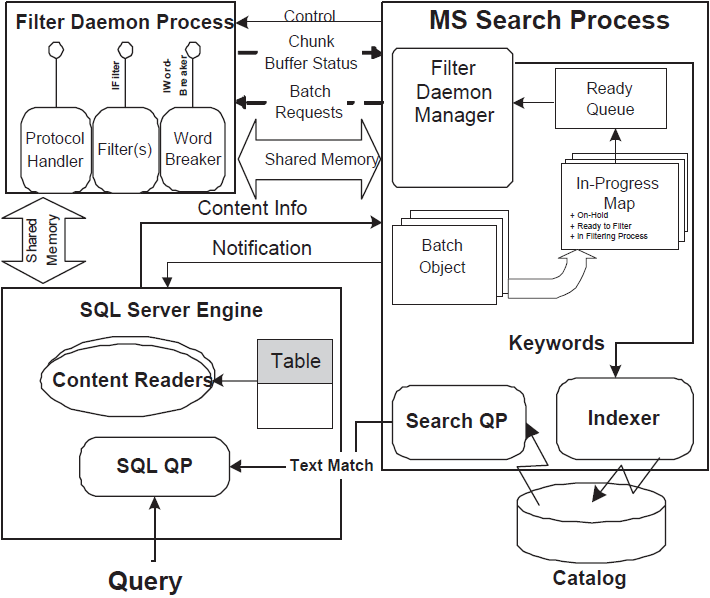
\includegraphics[width=0.9\textwidth]{sql_search_architecture.png}
    \\
    \cite[Source:][p. 8]{hamilton_microsoft_2001}
\end{figure}
\textbf{Word breakers} split the chunks into keywords and additionally provide alternative keywords and the corresponding position in the text. Word breakers can recognize human languages and on \ac{SQL} Server several word breakers for different languages are installed by default. The generated keywords and metadata are passed on to the \ac{MS} Search process, which processes the data with an indexer.\\
The \textbf{indexer} generates an inverted keyword list with a batch containing all keywords of one or more items. These indexes are compressed to use memory efficiently, this may lead to high costs for updates of these indexes. Therefore a stack of indexes is maintained. New documents first create their small indexes, which are regularly merged into a larger index, which in turn is merged into the base index. This stack can be deeper than three, but the concept remains and allows a strongly compressed index without driving the update costs too high. If a keyword is searched, all indexes are accessed, so the depth should still be kept reasonable.\\
A \textbf{query processor} manages the insertion and merge operations and collects statistics on distribution and frequency for ranking purposes and query execution \parencite[cf.][pp. 8-9]{hamilton_microsoft_2001}.
\subsubsection{MS SQL Server Full-Text Query Features}
Full-text indexes can be created on \ac{SQL} Servers with the \ac{DDL} statement \lstinline[language=SQL]$CREATE INDEX$ and can make use of other \ac{SQL} Server utilities; these include backup and restore and attachment of databases. There are three options to create and manage indexes on \ac{SQL} Servers. \textbf{Full Crawl} always rebuilds the whole full-text index by scanning the entire table. \textbf{Incremental Crawl} logs the timestamp of the last re-index and retains changes by storing them in a column. \textbf{Change Tracking} enables a near real-time validity between the full-text index and the table by tracking changes to the indexed data using the \ac{SQL} Server Query Processor \parencite[cf.][p. 9]{hamilton_microsoft_2001}.\\
Full-text search is represented in \ac{SQL} with three possible constructs: \parencite[cf.][p. 9]{hamilton_microsoft_2001}
\begin{enumerate}
    \item Contains Predicate: A contains predicate is true if one of the specified columns contains terms that satisfy the specified search condition. E.g. \lstinline[language=SQL]$Contains(author, ('Ag* or "Marc Miller"'))$ will match entries where the column author contains words like 'Ag', 'Agatha', or 'Marc Miller'.
    \item Freetext Predicate: Freetext predicates are true if one of the specified columns contains terms that stem from the terms in the specified search condition. E.g. \lstinline[language=SQL]$Freetext(content, 'fishing')$ will match entries where content contains words like 'fishing', 'fish', or 'fisher'.
    \item ContainsTable and FreetextTable: ContainsTable and FreetextTable are functions that match entries similar to their corresponding function, but additionally return multiple matches including a ranking for each entry and the entire corpus.
\end{enumerate}
The search conditions of these constructs can be of various types to find the intended results: \parencite[cf.][p. 9]{hamilton_microsoft_2001}
\begin{enumerate}
    \item Keyword, phrase, prefix: E.g. 'fishing', 'Marc Miller', 'Ag*'
    \item Inflections and Thesaurus: E.g. \lstinline[language=SQL]$Contains(*, 'FORMSOF(INFLECTIONAL, fishing) AND FORMSOF(THESAURUS, boat)')$ will find all entries containing words that stem from 'fishing' and all words sharing the meaning with 'boat' (Thesaurus support).
    \item Weighted terms: Keywords and phrases can be assigned a relative weight to impact the rank of entries. E.g. \lstinline[language=SQL]$ContainsTable(*, 'ISABOUT(generator weight (.7), full-text weight (.3))')$ will rank entries higher in the result corpus which mention 'generator' over 'full-text'.
    \item Proximity: E.g. \lstinline[language=SQL]$Contains(*, 'corn NEAR salad')$ contains the proximity term 'NEAR' to match entries where 'corn' appears close to 'salad'.
    \item Composition: E.g. \lstinline[language=SQL]$Contains(*, 'full-text AND NOT database')$ uses two search query components that are composed using a term like 'AND', 'OR', or 'AND NOT'.
\end{enumerate}

\subsection{Domain-Specific Languages}
Commonly known programming languages, such as C or Java, are also called a \ac{GPL}. \ac{GPL}s are designed to handle any problem with relatively equal levels of efficiency and expressiveness. However, many applications do not require a multifunctional \ac{GPL} and can describe a problem more naturally using a \ac{DSL}. \ac{DSL}s are languages that have been developed specifically for a particular application or domain, to be able to develop faster and more effectively \parencite[cf.][p. 1]{hudak_domain-specific_1997}. By tailoring notations and constructs to the domain in question, \ac{DSL}s offer significant gains in expressiveness and usability compared to \ac{GPL}s for the domain in question, with corresponding productivity gains and lower maintenance costs \parencite[cf.][p. 317]{mernik_when_2005}. \ac{DSL}s are by no means a product of modern software development but have existed since the beginning of programming. One of the first \ac{DSL}s ever designed was \ac{APT}, which was used for the development of numerically controlled machine tools in 1957 \parencite[cf.][pp. 283-284]{ross_origins_1978}.\\
\ac{DSL}s can be found everywhere in the world of IT, for example, this thesis was written with the help of \LaTeX{} to design layout and formatting. Table \ref{tbl:popular_dsl} lists some well-known \ac{DSL}s and their application/domain to give examples of what is classified as a \ac{DSL}.
\begin{table}[H]
    \caption{Popular DSLs}
    \label{tbl:popular_dsl}
    \begin{tabularx}{\textwidth}[ht]{|l|X|l|}
        \hline
        \textbf{DSL}         & \textbf{Applicaiton}                        \\
        \hline
        Lex and Yacc         & program lexing and parsing                  \\
        PERL                 & text/file manipulation/scripting            \\
        VDL                  & hardware description                        \\
        \TeX, \LaTeX, troff  & document layout                             \\
        HTML, SGML           & document markup                             \\
        SQL, LDL, QUEL       & databases                                   \\
        pic, postscript      & 2D graphics                                 \\
        Open GL              & high-level 3D graphics                      \\
        Tcl, Tk              & GUI scripting                               \\
        Mathematica, Maple   & symbolic computation                        \\
        AutoLisp/AutoCAD     & computer aided design                       \\
        Csh                  & OS scripting (Unix)                         \\
        IDL                  & component technology (COM/CORBA)            \\
        Emacs Lisp           & text editing                                \\
        Prolog               & logic                                       \\
        Visual Basic         & scripting and more                          \\
        Excel Macro Language & spreadsheets and many things never intended \\
        \hline
    \end{tabularx} \\
    \cite[Source:][p. 3]{hudak_domain-specific_1997}
\end{table}
Programs written in a \ac{DSL} are considered to be more concise, quicker to write, easier to maintain and easier to reason about and most importantly they can be written by non-programmers. In particular, experts in the domain for which the \ac{DSL} was developed can use \ac{DSL}s to program applications without having to acquire programming skills. An expert of a domain already knows the semantics of the domain, all that is needed to start development is the corresponding notation that expresses these semantics \parencite[cf.][pp. 2-4]{hudak_domain-specific_1997}.

\subsection{Building a language}
For a compiler or an interpreter to be able to interpret a \ac{DSL}, the language must be accurately and precisely defined. Accurately means that the language must be defined consistently down to the smallest detail. Precisely means in this case that all aspects of the language must be laid out. If parts of the language are inconsistent or too vague, authors of compilers are forced to interpret these aspects themselves. This inevitably leads to different authors having different approaches to the same problem. If a \ac{DSL} is to be created that meets the criteria described above, two components are needed. The first component is a set of rules, also called syntax. The second component is a formal definition of the meaning, also called semantics \parencite[cf.][file 2]{farrell_compiler_1995}.
\subsubsection{Syntax}
The first step when defining syntax is defining an alphabet. This alphabet consists of tokens, which do not necessarily have to be letters. Several tokens, formulated according to a set of rules, make up a sentence or string. The alphabet of the English language is, in the context of syntax, not a list of the permissible characters, which is predominantly called the alphabet or 'ABC', but the permissible tokens.
E.g. in the sentence 'the donkey screams' the tokens 'the', 'donkey' and 'screams' are part of the alphabet of the English language. The token 'gHArFk' consists of permissible characters but is not part of the valid alphabet. However, the use of permissible tokens alone does not make a sentence correct. The sentence 'on sleep blue' consists of tokens that are part of the English alphabet, but it is still not a valid sentence. The correct application of the rule set is still missing, in this example a missing object. Only the correct use of the alphabet AND the set of rules make a sentence syntactically correct \parencite[cf.][file 2]{farrell_compiler_1995}.\\
If the alphabet and the set of rules are notated in a normal form, they can be called grammar. Relevant to this thesis is the \ac{EBNF}, which will be described in section \ref{sec:EBNF}.
\subsubsection{Extended Backus-Naur Form}\label{sec:EBNF}
\ac{EBNF}, as the name suggests, is based on the Backus-Naur Form, which was proposed by a group of thirteen international representatives in 1960, to serve as a basic reference and guide for building compilers. Backus-Naur Form is a notation for describing computational processes and rules as arithmetic expressions, variables, and functions \parencite[cf.][p. 300]{backus_report_1960}.\\
The syntax can be described as a set of metalinguistic formulae best described with an example. The grammar describing a number can be written in Backus-Naur Form as:
\begin{grammar}
    <number> ::= <positive>|-<positive>|0 \\
    <positive> ::= <digit not zero><optional> \\
    <optional> ::= <digit><optional>| \\
    <digit> ::= <digit not zero>|0 \\
    <digit not zero> ::= 1|2|3|4|5|6|7|8|9
\end{grammar}
Characters contained in angel brackets '<>' represent a metalinguistic variable. The character '::=' describes a definition of this variable. The character '|' represents the metalinguistic connective 'or'. Other characters in this example have no special meaning but only represent themselves. So the first line of the grammar means that the variable <number> can be defined or replaced as <positive> or -<positive> or as 0. Since the variable <positive> is mentioned in the definition, there must be a definition for this variable in the grammar, otherwise, the grammar would be incomplete. In the third line, we see a metalinguistic connective without content on its right side. This means that the variable <optional> can also be empty and thus without value. Furthermore, in this line, a variable calls itself recursively, which is allowed \parencite[cf.][pp. 301-303]{backus_report_1960}.\\
So following this grammar, numbers such as 42 or -3141592 are valid.\\
In 1977 Wirth proposed a new variant of the Backus-Naur Form to further improve language definition notation. The main goals of this new notation were to \parencite[cf.][p. 822]{wirth_what_1977}
\begin{itemize}[noitemsep]
    \item distinguish clearly between metaterminal and nonterminal symbols
    \item not exclude metaterminals as possible symbols of the language
    \item enable iteration without using recursion
\end{itemize}
This proposal was the basis for the ISO/IEC 14977:1996(E) which now defines the standard for \ac{EBNF}. The major changes that \ac{EBNF} brought can be summarized as: \parencite[cf.][p. VI]{isoiec_149771996e_information_1996}
\begin{itemize}[noitemsep]
    \item Terminal symbols must be quoted so any symbol can be a terminal symbol of the language
    \item Added square brackets to indicate optional symbols and avoid the use of a <empty> symbol
    \item Added curly brackets to indicate repetition
    \item Every rule must have a final character
    \item Normal Brackets group items together, similar to their arithmetic use
\end{itemize}
The number example from above can be rewritten in \ac{EBNF} as:
\begin{grammar}
    <number> ::= (['-']<digit not zero>\{<digit>\})|'0'; \\
    <digit> ::= <digit not zero>|'0'; \\
    <digit not zero> ::= '1'|'2'|'3'|'4'|'5'|'6'|'7'|'8'|'9';
\end{grammar}
This version of the grammar produces the same set of numbers but is more concise and arguably more readable for humans.

\newpage
\section{Implementation}
When using the full-text search, large parts of the SQL statements needed to describe the search are the same, since the search criteria are defined as either WHERE conditions or JOIN criteria. To define a full-text search, usually use a combination of the given functions is used. In Transact-\ac{SQL} this would be for example CONTAINS or FORMSOF. Therefore the goal is to develop a query language where only a combination of functions and a few parameters is necessary to generate the corresponding SQL.
\subsection{Language definition}
The first step to defining a language is to define its purpose. In this case, there should be functions that represent full-text functions. Furthermore, one must be able to pass parameters to these functions and one should be able to combine both parameters and functions with logical operators and, or and not.
To announce a function, this query language uses an '@', e.g. '@contains'. From programming languages of the C-family one recognizes the use of parentheses '()' to define parameters. To avoid later confusion with parentheses used for logical grouping, this language uses the colon ':' to enclose parameters. For now, a parameter is defined as a simple word or phrase, which is delimited with quotes '"'. These few rules already allow the definition of a query, such as \lstinline[language=Fulltext-Search]$@contains:apple:$ where 'contains' is the name of a function.
This first set of rules can be written in \ac{EBNF} as:
\begin{grammar}
    <search> ::= '@'<function>':'<parameter>':'; \\
    <function> ::= 'contains'; \\
    <parameter> ::= <word>|' '' '\{[' ']<word>\}' '' '; \\
    <word> ::= \{'a'-'z'|'A'-'Z'\};
\end{grammar}
Note that the function variable only includes 'contains'. In future definitions, it should accept the different functions that are going to be defined.\\
A feature that is also needed is the logical combination and negation of multiple search terms. For example, it should be possible to search for 'apple' or 'tree' and not 'worm'. To represent AND the language accepts the characters '\&' and '+', for OR it accepts '|', and for negation it accepts '!' and '-'. To cover all possible logical operations, groups are also needed to allow precedence between the different operators. For this parentheses are used. Using groups it is now possible to build a logic like 'apple' AND NOT('tree' OR 'worm'), where the whole statement inside the parentheses is processed negated, and prioritized instead of simply being processed from left to right.\\
To cover a large part of the possible full-text search queries, six functions were finally selected which are to be implemented in the query language:\\
\textbf{Contains} should be a simple search for a search term or a combination of search terms.\\
\textbf{Startswith} searches for terms, which start with the given search term.\\
\textbf{Inflection} takes the given search terms and searches for words with the same root and variations of it.\\
\textbf{Thesaurus} uses a thesaurus to search for entries with the same meaning as the search terms.\\
\textbf{Near} can search for documents where two or more search terms must occur within a certain distance of each other. Distance in this case means how many words separate the search terms\\
\textbf{Weighted} enables the search for multiple search terms and assigns each a weight to allow certain terms to be prioritized.\\
Some of the functions require the definition of more possible parameters than just words and phrases. For the function Near a positive integer is needed to specify the distance and for Weighted positive decimal numbers between zero and one are needed to assign a weight to the search parameters. In addition, functions should also be combinable with operators.\\
These specifications and rules can be defined in \ac{EBNF} as follows:
\begin{grammar}
    <search> ::= <function>\{[<infix><function>]\}; \\
    <infix> ::= '+'|'\&'|'|'; \\
    <function> ::= '@'(<contains>|<startswith>|<inflection>|<thesaurus>|<near>|<weighted>); \\

    <contains> ::= 'contains:'<expression>':'; \\
    <startswith> ::= 'startswith:'<expression>':'; \\
    <inflection> ::= 'inflection:'<wordorphrase>':'; \\
    <thesaurus> ::= 'thesaurus:'<wordorphrase>':'; \\
    <near> ::= 'near:'<wordorphrase>\{','<wordorphrase>\}[','<posinteger>]':'; \\
    <weighted> ::= 'weighted:'\{<wordorphrase>','<zerotoone>\}':'; \\

    <expression> ::= <wordorphrase>[' '<wordorphrase>]|'('<expression>')'|('-'|'!')<expression>\\
    \hspace*{\fill}|<expression><infix><expression>; \\
    <wordorphrase> ::= <word>|' '' '\{[' ']<word>\}' '' '; \\
    <word> ::= \{'a'-'z'|'A'-'Z'\}; \\
    <posinteger> ::= \{'0'-'9'\}; \\
    <zerotoone> ::= \{0\}['.'\{'0'-'9'\}]|'1';
\end{grammar}
\subsection{Code Generator}
\subsubsection{Lexer}
The first part of a code generator is the lexer. A lexer gets a file or in this case a string as input and divides this input into a series of tokens. So the input \lstinline[language=Fulltext-Search]$@contains:apple:$ becomes the tokens: '@', 'contains', ':', 'apple', and ':'. These tokens are not interpreted yet but are only being recognized as separate characters. To achieve this in code the crate logos is used, to avoid writing redundant code. To understand the code written in lexer.rs what follows is a short explanation of how this crate is used in the context of this prototype.\\
To define tokens, Logos can be added to the derive statement of an enumeration and a matching rule can be defined using a literal string or a regular expression. For example, in line 73 of code listing \ref{code:tokens}, a literal string is used to recognize the colon token, and line 33 uses a regular expression to recognize decimals between 0 and 1. It also calls an arbitrary function to\_float (code \ref{code:tokens}, 17-19) to define that in this case the data should be cast into the datatype f64. Logos also requires an error type (code \ref{code:tokens}, 78-80), which is also used to skip whitespaces \parencite[cf.][n.p.]{hirsz_logos_2022}.
\begin{codeenv}
    \captionof{mycapcode}{Token definitions}
    \label{code:tokens}
    \lstinputlisting[language=Rust, linerange={16-19}]{code/code_gen/lexer.rs}
    \vdots
    \lstinputlisting[language=Rust, linerange={26-28}]{code/code_gen/lexer.rs}
    \vdots
    \lstinputlisting[language=Rust, linerange={32-34}]{code/code_gen/lexer.rs}
    \vdots
    \lstinputlisting[language=Rust, linerange={72-81}]{code/code_gen/lexer.rs}
    \centerline{Source: lexer.rs}
\end{codeenv}
These tokens are then compiled in a list and passed over to the parser as the work of the lexer is done.

\subsubsection{Parser}
In the parser, a large part of the heavy lifting is done, because here the list of tokens is interpreted and checked for their admissibility in the language. The parser of this custom query language stores a copy of the token list still to be parsed and additionally the current token and the next one in the list. The current token is often used to make comparisons between it and the token that would be expected, while the peek token is often used to see whether the end of the token list has already been reached. When initializing the parser both the current and the peek token are set to \lstinline[language=Rust]$Token::EoF$ which represents the edge case end of file (code \ref{code:parser-struct}, 66-67).
\begin{codeenv}
    \captionof{mycapcode}{Parser struct}
    \label{code:parser-struct}
    \lstinputlisting[language=Rust, linerange={54-69}]{code/code_gen/parser.rs}
    \centerline{Source: parser.rs}
\end{codeenv}
In the parsing process, two different levels are distinguished: expressions and statements. Statements are the various functions that can be used in the language, such as 'near', which is defined with several expressions as 'parameters' and another expression as a 'proximity' variable (code \ref{code:stat-expr}, 25-28). Expressions are the several values that can appear in a search query, for example, words, phrases, or numbers (code \ref{code:stat-expr}, 37-38). The special cases of operators are also represented by both statements and expressions. These will be discussed in more detail later.
\begin{codeenv}
    \captionof{mycapcode}{Statements and expressions}
    \label{code:stat-expr}
    \lstinputlisting[language=Rust, linerange={3-4}]{code/code_gen/ast.rs}
    \vdots
    \lstinputlisting[language=Rust, linerange={25-28}]{code/code_gen/ast.rs}
    \vdots
    \lstinputlisting[language=Rust, linerange={35-39}]{code/code_gen/ast.rs}
    \centerline{Source: ast.rs}
\end{codeenv}
The tokens are normally processed linearly, always watching out not to run past the end of the file (code \ref{code:read}, 74). With each call of read current and peek are updated and the next statement is parsed. Read is called manually twice at the beginning to overwrite the initial \lstinline[language=Rust]$Token::EoF$ (code \ref{code:read}, 12-14). Otherwise, the next statements are parsed until the end of the token list is reached (code \ref{code:read}, 16-18).
\begin{codeenv}
    \captionof{mycapcode}{Parser read}
    \label{code:read}
    \lstinputlisting[language=Rust, linerange={7-20}]{code/code_gen/parser.rs}
    \vdots
    \lstinputlisting[language=Rust, linerange={71-88}]{code/code_gen/parser.rs}
    \centerline{Source: parser.rs}
\end{codeenv}
When parsing a statement there must be a function token at the beginning of a statement (code \ref{code:weighted}, 120+140). If this token is found, the procedure is different depending on the function. For example, the function weighted is parsed as follows: (code \ref{code:weighted}, 325-355)\\
First, a colon is expected, because according to the language definition the parameters are introduced with one. As parameters, there are expected to be combinations of a search term (word or phrase) and a decimal between 0 and 1. These must be separated by commas. These tuples are expected until a colon appears as a token again. The decimals representing weights must add up to exactly 1. If none of the rules are violated, the list of tuples is passed back to the function parse\_statement and stored in the form of a statement enumeration (code \ref{code:weighted}, 140-142).
\begin{codeenv}
    \captionof{mycapcode}{Parse weighted}
    \label{code:weighted}
    \lstinputlisting[language=Rust, linerange={116-120}]{code/code_gen/parser.rs}
    \vdots
    \lstinputlisting[language=Rust, linerange={140-142}]{code/code_gen/parser.rs}
    \vdots
    \lstinputlisting[language=Rust, linerange={325-355}]{code/code_gen/parser.rs}
    \centerline{Source: parser.rs}
\end{codeenv}
In the parse\_statement function, two different functions are called to process tokens. On the one hand, expect\_token\_and\_read (code \ref{code:expect}, 110-114) compares the current token with an input variable and reads past it without further logic. This function is mostly used for parsing syntactic tokens, such as the colon, which themselves have no impact on the content of the search.
\begin{codeenv}
    \captionof{mycapcode}{expect\_token\_and\_read}
    \label{code:expect}
    \lstinputlisting[language=Rust, linerange={90-114}]{code/code_gen/parser.rs}
    \centerline{Source: parser.rs}
\end{codeenv}
The second function is parse\_expression, which is similar in logic to parse\_statement. Here the current token is compared to the possible expressions and returned as an expression enumeration. For example, with the WordOrPhrase token, the content is stored in the variable s and passed when the expression counterpart is generated (code \ref{code:parse-word}, 159-161).
\begin{codeenv}
    \captionof{mycapcode}{Parse WordOrPhrase}
    \label{code:parse-word}
    \lstinputlisting[language=Rust, linerange={156-162}]{code/code_gen/parser.rs}
    \centerline{Source: parser.rs}
\end{codeenv}
With these building blocks, it is already possible to parse a token list, like\\
\lstinline[language=Rust]$Near, Colon, WordOrPhrase("apple"), Comma, WordOrPhrase("tree"), Comma, Number(9), Colon$\\
into the statement\\
\lstinline[language=Rust]$Near{parameter: (WordOrPhrase("apple"), WordOrPhrase("tree")), proximity: Number(9)}$.\\
While parsing, attention has been paid to the syntax of the language and the information has been reduced to the minimum necessary in a structured way.

\subsubsection{Parsing Operators and Groups}\label{sec:operators}
In addition to simple search terms and the call of a single function, the query language should also offer the possibility to logically link search terms and use several functions simultaneously. To make this possible, operators such as AND, OR, and NOT, and groups come into play. To interpret these types of operators and groups and store them as part of the \ac{AST}, there are separate types for them as both statements and expressions. The statement enumeration (code \ref{code:op-enums}, 8-12) is used to allow the use of multiple functions in the query language, while the expression enumerations (code \ref{code:op-enums}, 40-41) are used to logically link search terms. The operators themselves are stored as a separate enumeration, with a function to translate tokens into operators (code \ref{code:op-enums}, 52-59).
\begin{codeenv}
    \captionof{mycapcode}{Operator statements and expressions}
    \label{code:op-enums}
    \lstinputlisting[language=Rust, linerange={3-12}]{code/code_gen/ast.rs}
    \vdots
    \lstinputlisting[language=Rust, linerange={33-36}]{code/code_gen/ast.rs}
    \vdots
    \lstinputlisting[language=Rust, linerange={40-60}]{code/code_gen/ast.rs}
    \centerline{Source: ast.rs}
\end{codeenv}
The big challenge with operators and groups is that it is no longer sufficient to process the token list linearly because operators are partly written after the affected tokens and hierarchies exist between the operators. For example, the AND operator has a stronger binding power than the OR operator, and groups, or parentheses, have an even higher binding power. This binding power is in text and code further called precedence.\\
Precedence is implemented as an ordered enumeration, which allows them to be compared and assigned higher or lower precedence. As with operators, there is a function to translate tokens into precedence (code \ref{code:precedence}, 37-51). The concept of precedence already appears in the code listings \ref{code:weighted} and \ref{code:parse-word} as an input variable for the functions parse\_statement and parse\_expression.
\begin{codeenv}
    \captionof{mycapcode}{Precedence}
    \label{code:precedence}
    \lstinputlisting[language=Rust, linerange={22-52}]{code/code_gen/parser.rs}
    \centerline{Source: parser.rs}
\end{codeenv}
Expression operators that are written before the token in question, such as the NOT operator, can be processed similarly to normal expressions. When the parser encounters one of the NOT tokens in parse\_expression (code \ref{code:not}, 171-177), an \lstinline[language=Rust]$Expression::Prefix$ is returned, where the actual search term is parsed with the parameter \lstinline[language=Rust]$Precedence::Prefix$, which is higher than the default \lstinline[language=Rust]$Precedence::Lowest$.
\begin{codeenv}
    \captionof{mycapcode}{Parse NOT}
    \label{code:not}
    \lstinputlisting[language=Rust, linerange={171-177}]{code/code_gen/parser.rs}
    \centerline{Source: parser.rs}
\end{codeenv}
More complicated are operators which are written after an affected token. For this, in parse\_expression after a token was parsed an attempt is made to parse a postfix or infix operator. At the same time, the precedence of the next token is compared to keep the corresponding hierarchies of the operators (code \ref{code:infix}, 189-197). The expression parsed so far is passed to the parse\_infix\_expression function and it structures it into an \lstinline[language=Rust]$Expression::Infix$, where the next search term is parsed again with the corresponding precedence.
\begin{codeenv}
    \captionof{mycapcode}{Parse infix operator}
    \label{code:infix}
    \lstinputlisting[language=Rust, linerange={188-197}]{code/code_gen/parser.rs}
    \vdots
    \lstinputlisting[language=Rust, linerange={220-238}]{code/code_gen/parser.rs}
    \centerline{Source: parser.rs}
\end{codeenv}
Postfix operators as such do not exist in the query language; instead, a search term written without an infix operator in between is parsed as a postfix AND (code \ref{code:postfix}, 203-218). So 'apple tree' is parsed as 'apple AND tree'. The second search term could potentially be negated, so the case 'apple -tree' is also covered and parsed as 'apple AND NOT tree'.
\begin{codeenv}
    \captionof{mycapcode}{Parse postfix operator}
    \label{code:postfix}
    \lstinputlisting[language=Rust, linerange={201-218}]{code/code_gen/parser.rs}
    \centerline{Source: parser.rs}
\end{codeenv}
Groups are delimited by parentheses and contain the highest precedence of all operators. Inside a group, an expression is expected (code \ref{code:group}, 360), which is then returned as soon as a right parenthesis is read. It should be emphasized that groups are not expressions, but only handle the included expression with higher precedence, so the inner expression itself is returned instead of some kind of group expression (code \ref{code:group}, 184).
\begin{codeenv}
    \captionof{mycapcode}{Parse groups}
    \label{code:group}
    \lstinputlisting[language=Rust, linerange={178-185}]{code/code_gen/parser.rs}
    \vdots
    \lstinputlisting[language=Rust, linerange={357-363}]{code/code_gen/parser.rs}
    \centerline{Source: parser.rs}
\end{codeenv}
Infix operators were also implemented at the statement level to allow multiple functions to be used in a single query. The logic is the same as that of code listing \ref{code:infix}, except that statements are processed instead of expressions.
\begin{codeenv}
    \captionof{mycapcode}{Parse infix operator in statements}
    \label{code:infix-stat}
    \lstinputlisting[language=Rust, linerange={145-152}]{code/code_gen/parser.rs}
    \vdots
    \lstinputlisting[language=Rust, linerange={240-258}]{code/code_gen/parser.rs}
    \centerline{Source: parser.rs}
\end{codeenv}
These are all the building blocks needed to parse the entirety of the query language. The result of the parser is a list of statements or \ac{AST}. This is now passed to the generator to generate SQL code from the logical sequence of operators and search terms.
\subsection{Generator}
The generator is the last step of the code generator because it does not convert the query language into bytecode or similar, but into another language, in this case, \ac{SQL}. For this purpose, the generator is similarly structured to the parser, except that it receives an \ac{AST} as input instead of output and generates a string from it.\\
In \ac{TSQL} there are two ways to initiate a full-text search. The use of predicates to specify criteria for the search in the WHERE clause of a query and the use of a CONTAINSTABLE or FREETEXTTABLE, which contains matching results and can be joined to the table to be searched. This generator uses a CONTAINSTABLE to represent all the functions offered by the query language in \ac{SQL}. This method is preferred to predicates because it allows getting a list of results, sorted by how much they match the search criteria, also called a rank. In addition, CONTAINSTABLE is preferred to FREETEXTTABLE, because FREETEXTTABLE is suitable for more fuzzy searches and less for searches that use defining functions to narrow down the results.\\
Based on these findings, a part of the SQL command can be preformulated with a few constants containing the metadata of the database (code \ref{code:sql-parts}, 7-10). So an INNER JOIN of the CONTAINSTABLE and the table to be searched is made, where the rank must be greater than five to weed out inaccurate matches (code \ref{code:sql-parts}, 29). From this, the title and rank are selected and sorted by rank in descending order. The top five results are then finally returned (code \ref{code:sql-parts}, 22). The exact specifications of the CONTAINSTABLE, which represent the search criteria, is the part that is filled by the generator (code \ref{code:sql-parts}, 26-28).
\begin{codeenv}
    \captionof{mycapcode}{Generate sql\_parts}
    \label{code:sql-parts}
    \lstinputlisting[language=Rust, linerange={6-10}]{code/code_gen/generator.rs}
    \vdots
    \lstinputlisting[language=Rust, linerange={20-29}]{code/code_gen/generator.rs}
    \centerline{Source: generator.rs}
\end{codeenv}
Similar to the parser, the generator stores the list of statements and additionally the current and next statements as attributes, where the peek statement is used to check the end of the list. On initialization current and peek are set to \lstinline[language=Rust]$Statement::EoF$ (code \ref{code:gen-struct}, 45-46).
\begin{codeenv}
    \captionof{mycapcode}{Generator struct}
    \label{code:gen-struct}
    \lstinputlisting[language=Rust, linerange={33-48}]{code/code_gen/generator.rs}
    \centerline{Source: generator.rs}
\end{codeenv}
The logic to iterate through the list is similar to that of the parser with the use of a next function which checks if the end of the list has already been reached (code \ref{code:write}, 52) and generates the next element if not and a write function which updates the current and peek attributes (code \ref{code:write}, 60-65).
\begin{codeenv}
    \captionof{mycapcode}{Generator write}
    \label{code:write}
    \lstinputlisting[language=Rust, linerange={50-66}]{code/code_gen/generator.rs}
    \centerline{Source: generator.rs}
\end{codeenv}
In the code, three functions are used to generate all elements of an \ac{AST}. Similar to the parser, a distinction is made between statements and expressions and additionally operators.\\
The generate\_statement function is passed a statement to be generated (code \ref{code:gen-weight}, 71). Usually, this statement is one of the implemented functions of the query language, for example, weighted. In the case of the weighted function, the stored attribute 'parameter' is used to translate the statement into \ac{SQL} as follows. First, the \ac{SQL} function ISABOUT is called and a parenthesis is opened (code \ref{code:gen-weight}, 136). Then, for each tuple of search terms and their weights, the values are written down so that, for example, the values 'apple' and 0.4 give \lstinline[language=SQL]$apple WEIGHT (0.4),$ (code \ref{code:gen-weight}, 137-142). Finally, the last comma is deleted, the parenthesis of ISABOUT is closed, and all parts are combined into one string and returned(code \ref{code:gen-weight}, 143-145+150).
\begin{codeenv}
    \captionof{mycapcode}{Generate weighted}
    \label{code:gen-weight}
    \lstinputlisting[language=Rust, linerange={68-72}]{code/code_gen/generator.rs}
    \vdots
    \lstinputlisting[language=Rust, linerange={133-146}]{code/code_gen/generator.rs}
    \vdots
    \lstinputlisting[language=Rust, linerange={148-151}]{code/code_gen/generator.rs}
    \centerline{Source: generator.rs}
\end{codeenv}
There is a special case in generate\_statement, infix operators, this case calls generate\_statement for the two statements and generate\_operator for the operator (code \ref{code:gen-in-stat}, 79-81) and combines the results.
\begin{codeenv}
    \captionof{mycapcode}{Generate infix operator statements}
    \label{code:gen-in-stat}
    \lstinputlisting[language=Rust, linerange={73-84}]{code/code_gen/generator.rs}
    \centerline{Source: generator.rs}
\end{codeenv}
In the example above for generating weighted, the generate\_expression function was called in code listing \ref{code:gen-weight} in lines 138 and 139 to generate the search terms and weights. This function takes as input the expression it should generate and returns the value of the expression as a string if a normal expression was passed (code \ref{code:gen-expr}, 158-160).
\begin{codeenv}
    \captionof{mycapcode}{Generate expressions}
    \label{code:gen-expr}
    \lstinputlisting[language=Rust, linerange={153-160}]{code/code_gen/generator.rs}
    \vdots
    \lstinputlisting[language=Rust, linerange={186-188}]{code/code_gen/generator.rs}
    \centerline{Source: generator.rs}
\end{codeenv}
If a form of an operator is passed as an expression, the corresponding generate function is called for the operators (code \ref{code:gen-op-expr}, 167+181) and the respective expressions are passed to the generate\_expression function. In the case of infix operators, parentheses are also set to safely represent the precedence as recognized by the parser (code \ref{code:gen-op-expr}, 164-170).\\
Something to pay attention to in \ac{SQL} is that if a NOT operator follows an infix operator, it must be written before the parenthesis, otherwise, \ac{SQL} throws a syntax error. To cover this case, infix operator generation checks if the second expression is a negation and rewrites the string in that case (code \ref{code:gen-op-expr}, 173-176).
\begin{codeenv}
    \captionof{mycapcode}{Generate operator expressions}
    \label{code:gen-op-expr}
    \lstinputlisting[language=Rust, linerange={161-185}]{code/code_gen/generator.rs}
    \centerline{Source: generator.rs}
\end{codeenv}
The third and simplest generate function is generate\_operator, which translates operators into a string (code \ref{code:gen-op}, 195-196). Noticeable here is the NOT operator, which is already treated separately in code listing \ref{code:gen-op-expr} lines 173-176.
\begin{codeenv}
    \captionof{mycapcode}{Generate operators}
    \label{code:gen-op}
    \lstinputlisting[language=Rust, linerange={190-201}]{code/code_gen/generator.rs}
    \centerline{Source: generator.rs}
\end{codeenv}
All parts up to the generator combined already make up a working code generator for a custom query language. For example the input \lstinline[language=Fulltext-Search]$@contains:apple -tree: + @thesaurus:"human":$, the lexer converts into a list of tokens. The parser then interprets these tokens into an \ac{AST}, one exemplary representation can be seen in figure \ref{fig:ast-example}.
\begin{figure}[H]
    \caption{Parsed example AST}
    \label{fig:ast-example}
    \begin{forest}
        box/.style={sharp corners,
        draw=gray!50,
        fill=gray!20,
        },
        for tree={box,align=center,minimum width=80pt}
            [{Infix\\AND}
                    [Contains
                            [{Infix\\AND}
                                    [{WordOrPhrase\\apple}]
                                    [{Prefix\\NOT}
                                            [{WordOrPhrase\\tree}]
                                    ]
                            ]
                    ]
                    [Thesaurus
                            [{WordOrPhrase\\"human"}]
                    ]
            ]
    \end{forest}
    \\
    \centerline{Source: Own representation}
\end{figure}
The generator then takes the \ac{AST} and generates from it the \ac{SQL} in code listing \ref{code:sql-example}. Lines 1 to 9 and 11 to 14 are the more or less pre-formulated part using the constants of the test database. Line 10 is the intriguing part, which is generated from the passed functions and search criteria.
\begin{codeenv}
    \captionof{mycapcode}{Generated example SQL}
    \label{code:sql-example}
    \begin{lstlisting}[language=SQL]
USE Wikipedia;
SELECT TOP 5 *
FROM(
        SELECT FT_TBL.Title,
            KEY_TBL.RANK
        FROM [dbo].[Article] AS FT_TBL
            INNER JOIN CONTAINSTABLE(
                [dbo].[Article],
                *,
                ' ( apple ) AND NOT ( tree ) AND FORMSOF(THESAURUS,"human") '
            ) AS KEY_TBL ON FT_TBL.[ID] = KEY_TBL.[KEY]
        WHERE KEY_TBL.RANK > 5
    ) AS FS_RESULT
ORDER BY FS_RESULT.RANK DESC;
    \end{lstlisting}
    \centerline{Source: Own code generator}
\end{codeenv}
\subsection{Website as User Interface}
To interact with the code generator a website is used as an interface. To create a simple website the Rust crate actix\_web is used, which provides a web framework for Rust, and the crate tera, which enables the use of templates to quickly create a working frontend.\\
To host a website using actix\_web, an HTTP server must be started in an asynchronous main function \parencite[cf.][n.p.]{ede_actix_2022}. With the help of tera, HTML templates can now be used \parencite[cf.][n.p.]{prouillet_tera_2022} to pass data to the server (code \ref{code:main}, 20+22). The HTML code of the website can be found in the appendix. The HTTP server hosts two subpages (code \ref{code:main}, 23-24). These are the start page, where a search query can be submitted, and the result page, where the search results will be displayed.
\begin{codeenv}
    \captionof{mycapcode}{HTTP Server}
    \label{code:main}
    \lstinputlisting[language=Rust, linerange={15-29}]{code/code_gen/main.rs}
    \centerline{Source: main.rs}
\end{codeenv}
The interface between the website and Rust code serves two structs, which can exchange data between the two parties. For this purpose, the crate serde is used, with which structs can be easily serialized \parencite[cf.][n.p.]{tolnay_serde_2017}. A struct for the search query including a string is needed (code \ref{code:web-search}, 114-117), and a struct for the search results, which contain a title and link as a string and a rank as an unsigned integer each (code \ref{code:web-search}, 118-123).\\
Each of the subpages is assigned a function, which defines for the respective page, what functionally happens on it. The search page is straightforward, with a text field that can be submitted (code \ref{code:web-search}, 125-131).
\begin{codeenv}
    \captionof{mycapcode}{Website search}
    \label{code:web-search}
    \lstinputlisting[language=Rust, linerange={113-131}]{code/code_gen/main.rs}
    \centerline{Source: main.rs}
\end{codeenv}
The function of the result page is a bit more complex because here the code generator is run, the \ac{SQL} is executed and the results are read. Because the result page resembles a POST request the function is passed the data of the search page. From this, the search query is extracted and the code generator is executed (code \ref{code:web-result}, 138). With the help of two functions, the generated \ac{SQL} is executed and the results are read (code \ref{code:web-result}, 141-142).\\
The results of the query are in the form of a string-integer tuple and are now fitted into the form of the result struct (code \ref{code:web-result}, 146-153). The link attribute is very similar to the title, but all blanks are replaced with \_ so that this attribute can be used to link directly to the associated Wikipedia article, a small quirk of the chosen test data.
\begin{codeenv}
    \captionof{mycapcode}{Website results}
    \label{code:web-result}
    \lstinputlisting[language=Rust, linerange={133-156}]{code/code_gen/main.rs}
    \vdots
    \lstinputlisting[language=Rust, linerange={175-178}]{code/code_gen/main.rs}
    \centerline{Source: main.rs}
\end{codeenv}
More specifications about the build and display of the website can be found in the appendix in the HTML files.
\newpage
\section{Summary}
Summary


%-----------------------------------
% Appendix / Anhang
%-----------------------------------
\newpage
\section*{\AppendixName} %Überschrift "Anhang", ohne Nummerierung
\addcontentsline{toc}{section}{\AppendixName} %Den Anhang ohne Nummer zum Inhaltsverzeichnis hinzufügen

\begin{appendix}
	% Nachfolgende Änderungen erfolgten aufgrund von Issue 163
	\makeatletter
	\renewcommand\@seccntformat[1]{\csname the#1\endcsname:\quad}
	\makeatother
	\addtocontents{toc}{\protect\setcounter{tocdepth}{0}} %
	\renewcommand{\thesection}{\AppendixName\ \arabic{section}}
	\renewcommand\thesubsection{\AppendixName\ \arabic{section}.\arabic{subsection}}
	\apxtitle{Cargo.toml}
\lstinputlisting[language=toml]{code/code_gen/Cargo.toml}
\apxtitle{main.rs}
\lstinputlisting[language=Rust]{code/code_gen/main.rs}
\apxtitle{lexer.rs}
\lstinputlisting[language=Rust]{code/code_gen/lexer.rs}
\apxtitle{parser.rs}
\lstinputlisting[language=Rust]{code/code_gen/parser.rs}
\apxtitle{ast.rs}
\lstinputlisting[language=Rust]{code/code_gen/ast.rs}
\apxtitle{generator.rs}
\lstinputlisting[language=Rust]{code/code_gen/generator.rs}
\apxtitle{mod.rs}
\lstinputlisting[language=Rust]{code/code_gen/mod.rs}
\apxtitle{base.html}
\lstinputlisting[language=HTML]{code/code_gen/base.html}
\apxtitle{search.html}
\lstinputlisting[language=HTML]{code/code_gen/search.html}
\apxtitle{result.html}
\lstinputlisting[language=HTML]{code/code_gen/result.html}
\apxtitle{convert\_wiki\_to\_csv.py}
\lstinputlisting[language=Python]{code/wikidump_sqlserver/convert_wiki_to_csv.py}
\apxtitle{create\_article.sql}
\lstinputlisting[language=SQL]{code/wikidump_sqlserver/create_article.sql}
\apxtitle{create\_view.sql}
\lstinputlisting[language=SQL]{code/wikidump_sqlserver/create_view.sql}
\apxtitle{bulk\_insert.sql}
\lstinputlisting[language=SQL]{code/wikidump_sqlserver/bulk_insert.sql}
\end{appendix}
\addtocontents{toc}{\protect\setcounter{tocdepth}{2}}

%-----------------------------------
% Literaturverzeichnis
%-----------------------------------
\newpage
\printbibliography[heading=bibintoc,title={\langde{Literaturverzeichnis}\langen{Bibliography}}]

\newpage
\pagenumbering{gobble} % Keine Seitenzahlen mehr

%-----------------------------------
% Ehrenwörtliche Erklärung
%-----------------------------------
\section*{%
  \langde{Ehrenwörtliche Erklärung}
  \langen{Declaration in lieu of oath}}
\langde{Hiermit versichere ich, dass die vorliegende Arbeit von mir selbstständig und ohne unerlaubte Hilfe angefertigt worden ist, insbesondere dass ich alle Stellen, die wörtlich oder annähernd wörtlich aus Veröffentlichungen entnommen sind, durch Zitate als solche gekennzeichnet habe. Ich versichere auch, dass die von mir eingereichte schriftliche Version mit der digitalen Version übereinstimmt. Weiterhin erkläre ich, dass die Arbeit in gleicher oder ähnlicher Form noch keiner Prüfungsbehörde/Prüfungsstelle vorgelegen hat. Ich erkläre mich damit einverstanden, dass die Arbeit der Öffentlichkeit zugänglich gemacht wird. Ich erkläre mich damit einverstanden, dass die Digitalversion dieser Arbeit zwecks Plagiatsprüfung auf die Server externer Anbieter hochgeladen werden darf. Die Plagiatsprüfung stellt keine Zurverfügungstellung für die Öffentlichkeit dar.}
\langen{I hereby declare that I produced the submitted paper with no assistance from any other party and without the use of any unauthorized aids and, in particular, that I have marked as quotations all passages which are reproduced verbatim or near-verbatim from publications. Also, I declare that the submitted print version of this thesis is identical with its digital version. Further, I declare that this thesis has never been submitted before to any examination board in either its present form or in any other similar version. I herewith agree that this thesis may be published. I herewith consent that this thesis may be uploaded to the server of external contractors for the purpose of submitting it to the contractors’ plagiarism detection systems. Uploading this thesis for the purpose of submitting it to plagiarism detection systems is not a form of publication.}


\par\medskip
\par\medskip

\vspace{5cm}

\begin{table}[H]
	\centering
	\begin{tabular*}{\textwidth}{c @{\extracolsep{\fill}} ccccc}
		\myOrt, \the\day.\the\month.\the\year
		&
		% Hinterlege deine eingescannte Unterschrift im Verzeichnis /abbildungen und nenne sie unterschrift.png
		% Bilder mit transparentem Hintergrund können teils zu Problemen führen
		
\includegraphics[width=0.35\textwidth]{unterschrift}\vspace*{-0.35cm}
		\\
		\rule[0.5ex]{12em}{0.55pt} & \rule[0.5ex]{12em}{0.55pt} \\
		\langde{(Ort, Datum)}\langen{(Location, Date)} & \langde{(Eigenhändige Unterschrift)}\langen{(handwritten signature)}
		\\
	\end{tabular*} \\
\end{table}

\end{document}
